\icode{N23X-EME-SI-L2-261121-002}
\nceeID[4]{2023湖南}{5}
如图，真空中有三个点电荷固定在同一直线上，电荷量分别为\(Q_1\)、\(Q_2\)、\(Q_3\)，\(P\)点和三个点电荷的连线与点电荷所在直线的夹角分别为\qty{90}{\degree}、\qty{60}{\degree}和\qty{30}{\degree}。若\(P\)点处的电场强度为零，\(q > 0\)，则三个点电荷的电荷量可能为\paren[]

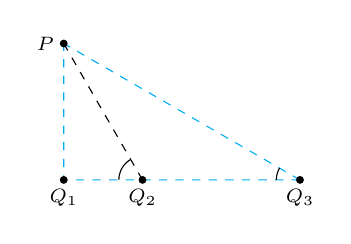
\begin{tikzpicture}[>=stealth,font=\scriptsize]
	\draw[dashed,cyan] (0,0)--(150:{2*sqrt(3)}) (0,0)--(-3,0)--(-3,{sqrt(3)});
	\draw[dashed,xshift=-2cm] (0,0)--(120:2);
	\fill (-3,{sqrt(3)})node[left]{\(P\)} circle(.05);
	\fill (-3,0)node[below]{\(Q_1\)} circle(.05);
	\fill (-2,0)node[below]{\(Q_2\)} circle(.05);
	\fill (0,0)node[below]{\(Q_3\)} circle(.05);
	\draw (-.3,0) arc(180:150:.3);
	\draw[xshift=-2cm] (-.3,0) arc(180:120:.3);
\end{tikzpicture}
\begin{choices}
	\item \(Q_1 = q\)、 \(Q_2 = \sqrt{2}q\)、 \(Q_3 = q\)
	\item \(Q_1 = -q\)、 \(Q_2 = -\frac{4 \sqrt{3}}{3}q\)、 \(Q_3 = - 4q\)
	\item \(Q_1 = -q\)、 \(Q_2 = \sqrt{2}q\)、 \(Q_3 = -q\)
	\item \(Q_1 = q\)、 \(Q_2 = - \frac{4\sqrt{3}}{3}q\)、 \(Q_3 = 4q\)
\end{choices}
\begin{answer}
	
\end{answer}